While tiling itself is a well-known optimization technique, we must consider the parts of why it works.
Temporal locality is increased because the scope of the work is smaller, which is done by sacraficing a bit of spatial locality: we no longer load an entire row, only a part.
However, this only explains the horizontal tiling, vertical tiling only reduces the scope as we work on a smaller tile but when considering the entire workload, it ultimately does not matter.
It can even be argued that by tiling vertically, we fragment the the workload as temporal locality cannot be guaranteed between tiles.

\section{Theory}
\label{sec:implementation_theory}

In a sense, grouping columns is similar to striding clusters of data, except in the case when a row of work can't be perfectly strided.
When the width of a multidimensional array is not a multiple of the stride, the loads will not align column wise (figure \ref{fig:column_vs_striding}).
To work around this, in the column approach we allow the last column to be narrower.

\begin{figure}[!hb]
    \centering
    
    \subfloat[Striding does not work well when the width of the task is a non-multiple of the striding factor.]{
        \centering
        \makebox[0.4\columnwidth][c]{
            \begin{tikzpicture}[scale=0.25, decoration = {
                markings, mark = between positions 0.3cm and 0.95 step 0.25cm with {\arrow{stealth}}
            }]
                \fill[gray]    (0, 3) rectangle +(4, 1);
                \fill[gray!50] (4, 3) rectangle +(4, 1);
                \fill[gray]    (8, 3) rectangle +(3, 1);

                \fill[gray]    (0, 2) rectangle +(1, 1);
                \fill[gray!50] (1, 2) rectangle +(4, 1);
                \fill[gray]    (5, 2) rectangle +(4, 1);
                \fill[gray!50] (9, 2) rectangle +(2, 1);

                \fill[gray!50] (0, 1) rectangle +(2, 1);
                \fill[gray]    (2, 1) rectangle +(4, 1);
                \fill[gray!50] (6, 1) rectangle +(4, 1);
                \fill[gray]    (10, 1) rectangle +(1, 1);

                \fill[gray]    (0, 0) rectangle +(3, 1);
                \fill[gray!50] (3, 0) rectangle +(4, 1);
                \fill[gray]    (7, 0) rectangle +(4, 1);

                \draw[step=1,gray!25] (0, 0) grid (11, 4);
            \end{tikzpicture}
        }
        \label{fig:striding_misalignment}
    }
    \qquad
    \subfloat[Allowing the last column to be flexible allows columns of thread groups to stay cohesive.]{
        \centering
        \makebox[0.4\columnwidth][c]{
            \begin{tikzpicture}[scale=0.25, decoration = {
                markings, mark = between positions 0.3cm and 0.95 step 0.25cm with {\arrow{stealth}}
            }]
                \fill[gray]    (0, 3) rectangle +(4, 1);
                \fill[gray!50] (4, 3) rectangle +(4, 1);
                \fill[gray]    (8, 3) rectangle +(3, 1);

                \fill[gray!50] (0, 2) rectangle +(4, 1);
                \fill[gray]    (4, 2) rectangle +(4, 1);
                \fill[gray!50] (8, 2) rectangle +(3, 1);

                \fill[gray]    (0, 1) rectangle +(4, 1);
                \fill[gray!50] (4, 1) rectangle +(4, 1);
                \fill[gray]    (8, 1) rectangle +(3, 1);

                \fill[gray!50] (0, 0) rectangle +(4, 1);
                \fill[gray]    (4, 0) rectangle +(4, 1);
                \fill[gray!50] (8, 0) rectangle +(3, 1);

                \draw[step=1,gray!25] (0, 0) grid (11, 4);
            \end{tikzpicture}
        }
        \label{fig:column_alignment}
    }
    \caption{
        Striding does not work if the stride does not fit perfectly in the input width. Flexibility is required.
    }
    \label{fig:column_vs_striding}
\end{figure}

\noindent
The index mapping $i \mapsto j$ to get the columning order consists out of four parts (figure \ref{fig:column_remap_parts}):
\begin{itemize}
    \item The starting offset of the column $o$.
    \item The column width $w'$.
    \item The index within a column $i'$.
    \item The position within the column $(x, y)$.
\end{itemize}

\begin{figure}[!hb]
    \centering
    \begin{tikzpicture}
        % offset
        \node at (2, 0.5) {offset $o$};
        \draw[decorate, thick, decoration={brace}] (0.1,0.1) --  (3.9,0.1);

        % x
        \node at (5.5, 0.5) {$x$ pos. in column};
        \draw[decorate, thick, decoration={brace}] (4.1,0.1) --  (6.9,0.1);

        % y
        \node [rotate=90] at (-0.5, -1.5) {$y$ pos. in column};
        \draw[decorate, thick, decoration={brace}] (-0.1,-2.9) -- (-0.1,-0.1);

        % current column:
        \draw[gray, pattern=north east lines, pattern color=gray!50] (4,0) rectangle (8, -6);

        % input array:
        \draw (0, 0) rectangle (12, -6);

        \draw[loosely dotted, very thick] (7, 0) -- (7,-6);
        \draw[loosely dotted, very thick] (0, -3) -- (12,-3);

        \foreach \i in {0.5,1.0,...,5} {
            \draw[gray, ->-] (4.5,-\i) -- (7.5,-\i);
            \draw[gray, ->-, dashed] (7.5,-\i) -- (4.5,-\i - 0.5);
        }
        \draw[gray, ->-] (4.5,-5.5) -- (7.5,-5.5);
        
        \node[fill, circle, label={[fill=white]above right:$i' \mapsto j$}] at (7, -3) {};

    \end{tikzpicture}
    \caption{
        The anatomy of the column based index remapping.
    }
    \label{fig:column_remap_parts}
\end{figure}

First, we calculate the offset for the starting index of the column we need to map to:

\begin{align}
    o  &= \floor{\frac{i}{I_h w}} w
    \\ \intertext{Then, modify the width value such that the last column does not exceed the input width:}
    w' &= \begin{cases}
        I_w - o& \text{if last column}
        \\
        w & \text{otherwise}
    \end{cases}
    \\ \intertext{And take $i'$ as the index within a column:}
    i' &= i \bmod I_h w'
    \\ \intertext{Calculate the position $(x, y)$ within the column:}
    x & = i' \bmod w'
    \\ 
    y & = \floor{\frac{i'}{w'}}
    \\ \intertext{So that we can calculate $j$:}
    \label{eq:column_mapping_to_j}
    j  &= x + y I_w + o
\end{align}

On GPUs threads in threadblocks are batched in warps of 32 threads and these warps may be executed in an arbitrary order (section \ref{sec:kernel_execution}).
As a result we might not be able to exploit the cache as much since column orders are highly dependent on thread order and on the higher level, CTAs may be assigned in a completely arbitrary way.

\subsection{Zigzagging variation}
When working in warps of 32-threads and having a non-multiple of 32 wide columns, the workload for a warp may be spread out due to the tail end of our task being put at the beginning of the next row.
By reversing the order of every other row, we can keep accesses local to each other when they span multiple rows.
We can modify equation \ref{eq:column_mapping_to_j}:

\begin{equation}
    j = \left(\begin{cases}
        x & y \text{ is uneven}
        \\
        w' - x & y \text{ is even}
    \end{cases}\right)  + y I_w + o
\end{equation}

\subsection{Higher dimensions}
Since works only gets split horizontally, namely the one dimension that benefits from spatial locality, this algorithm can work on higher dimensions.
All other dimensions can only exploit temporal locality and do not benefit from spatial locaity.
We can therefore encapsulate an N-dimensional problem into 2-dimensional (horziontal and vertical) one, by mapping all but the first dimension to the vertical dimension.

\section{Implementation}

The remapping algorithm described in section \ref{sec:implementation_theory} can be directly transcribed into C code (listing \ref{lst:column_cuda}).
Note that we use a minimum operator on line 35 instead of a condition the avoid branching.

\begin{listing}[ht]
    \begin{minted}{cuda}
__global__ void my_kernel(int width, [...]){
    // For a given thread ID we can compute the 
    // new thread ID and it's x, y position:
    int tid = blockIdx.x * blockDim.x + threadIdx.x;
    int x; // originally x = tid % width;
    int y; // originally y = tid / width;

    if (tid >= width * height) {
        return;
    }

    int col_size = height * col_w;

    // Column identifier
    int col_id  = tid / col_size;

    // Thread id within column
    int col_tid = tid % col_size;

    // Column offset
    int col_off = col_id * col_w;

    // True width of column
    //
    // int col_tw  = col_w;
    // if (col_id == width  / col_w) {
    //     col_tw  = width - col_id * col_w;
    // }
    //
    // A shorter version of  the above since col_tw is 
    // always bounded by col_w. It removes the need of 
    // an expensive  divide operation  and saves 2 PTX
    // instructions overal. 
    
    int col_tw = min(width - col_id * col_w, col_w);

    x = (col_tid % col_tw) + col_off;
    y =  col_tid / col_tw;
    tid = x + (y * width);

    do_things_with(tid, x, y);
}
    \end{minted}
    \caption{
        The CUDA C++ implementation column based remapping.
    }
    \label{lst:column_cuda}
\end{listing}

For the implementation in Accelerate, we first define the type signature of a thread id mapping function (listing {\ref{lst:threadmapping_type}}).
It takes the size of the task (\texttt{ShapeR sh} and \texttt{Operands sh}), the  original thread index (\texttt{Operands Int}) and produces the machinecode to compute the new thread index (\texttt{CodeGen arch (Operands Int)}).
\begin{listing}[!ht]
    \begin{minted}{haskell}    
type ThreadMapping sh e arch 
    =  ShapeR sh 
    -> Operands sh 
    -> Operands Int 
    -> CodeGen arch (Operands Int)
    \end{minted}
    \caption{
        The type signature of a thread remapping function which takes the input dimension sizes and thread index and produces a new thread index.
    }
    \label{lst:threadmapping_type}
\end{listing}
We then implement the algorithm as described in section \ref{sec:implementation_theory} (listing \ref{lst:column_mapping})
\begin{listing}[ht]
    \begin{minted}{haskell}
column :: Operands Int -> ThreadMapping sh e arch
column column_width shr sh index = do
    -- input sizes
    input_width  <- widthOp shr sh
    input_size   <- sizeOp  shr sh
    input_height <- input_size |//| input_width
    
    column_size  <- column_width |*|  input_height
    column_count <- ((input_size |+| column_size) |-| (1::Int)) |//| column_size

    column_index      <- index |//| column_size
    column_last_index <- column_count |-| (1::Int)
    column_offset     <- column_index |*| column_width

    index' <- index |%| column_size

    column_current_width <- ifThenElse (
        TupRsingle $ SingleScalarType $ NumSingleType (numType @Int), 
        column_index |==| column_last_index
      ) ( do
        input_width |-| (column_last_index |*| column_width)
      ) ( do
        return column_width
      )
    
    x_in_column <- index' |%|  column_current_width
    y_in_column <- index' |//| column_current_width
    result      <- x_in_column |+| (y_in_column |*| input_width) |+| column_offset

    return result
    \end{minted}
    \caption{
        The thread remapping function for Accelerate implemented in Haskell.
    }
    \label{lst:column_mapping}
\end{listing}
However, in Accelerate a single thread can work on multiple elements if the work is larger than the maximum number of threads.
Part of the calculation can be moved out of the loop in the thread that handles the multiple elements to avoid unneeded work.
Instead of computing the complete remap every new index, we can precompute part of the algorithm (listing \ref{lst:column_mapping_precompute}).
This precomputation is done by calling \texttt{precomp\_column}.
The function returns a lambda (listing \ref{lst:column_mapping_precompute}, lines 16-34) that generates the machine code for the new index given the old index which can be called within the loop that enumerates over the elements.

\begin{listing}[ht]
    \begin{minted}{haskell}
precomp_column :: Operands Int 
               -> ShapeR sh 
               -> Operands sh 
               -> CodeGen arch (Operands Int -> CodeGen arch (Operands Int))
precomp_column column_width shr sh = do
    -- input sizes
    input_width  <- widthOp shr sh
    input_size   <- sizeOp  shr sh
    input_height <- input_size |//| input_width
    
    column_size  <- column_width |*|  input_height
    column_count <- ((input_size |+| column_size) |-| (1::Int)) |//| column_size

    column_last_index <- column_count |-| (1::Int)

    return \index -> do
        column_index  <- index |//| column_size
        column_offset <- column_index |*| column_width
        index' <- index |%| column_size

        column_current_width <- ifThenElse (
            TupRsingle $ SingleScalarType $ NumSingleType (numType @Int), 
            column_index |==| column_last_index
        ) ( do
            input_width |-| (column_last_index |*| column_width)
        ) ( do
            return column_width
        )
        
        x_in_column <- index' |%|  column_current_width
        y_in_column <- index' |//| column_current_width
        result      <- x_in_column |+| (y_in_column |*| input_width) |+| column_offset

        return result
    \end{minted}
    \caption{
        The column mapping from listing \ref{lst:column_mapping} with precomputing the fixed parameters.
    }
    \label{lst:column_mapping_precompute}
\end{listing}

\section{Stencil Operation}

The naive stencil operations had problems of chasing the cache on sufficiently large input sizes which tiling does resolve (section \ref{sec:stencil_tiled}).
Consider what the tiling implies: we split the work on all axis, to improve locality.
However, all tiling except horizontal is can be considered unnecessary because vertical tiling only causes to fragmentize the workload.

Let us first consider the single threaded case of column based iteration: by controlling the column width we can force the ideal scenario of the naive stencil implementation (figure \ref{fig:stencil_naive_loading_pattern_ideal}) to occur, similarly to tiling.
The column based approach is similar to tiling, but also allows the ideal memory access pattern to continue accross tiles vertically.
In GPUs this translates to less cohesive threads as threadblocks get assigned in a round-robin fashion to SMs, eliminating posibilities of L1 cache reuse.

\begin{figure}[!hb]
    \centering
    
    \subfloat[Grouping by column only incurs a heavy load every time a new column is started.]{
        \centering
        \makebox[0.4\columnwidth][c]{
            \begin{tikzpicture}[scale=0.25, decoration = {
                markings, mark = between positions 0.3cm and 0.95 step 0.25cm with {\arrow{stealth}}
            }]
                \fill[gray!50]  (-1, -1) rectangle +(6, 4);
                \fill[gray!15] (3, 6) rectangle +(3, 3);

                \draw[step=1,gray!25] (-1, -1) grid (9, 9);

                \draw[gray, postaction = decorate] (0.5, 7.5) -- +(3, 0);
                \draw[gray, dashed] (3.5, 7.5) -- +(-3, -1);
                \draw[gray, postaction = decorate] (0.5, 6.5) -- +(3, 0);
                \draw[gray, dashed] (3.5, 6.5) -- +(-3, -1);
                \draw[gray, postaction = decorate] (0.5, 5.5) -- +(3, 0);
                \draw[gray, dashed] (3.5, 5.5) -- +(-3, -1);
                \draw[gray, postaction = decorate] (0.5, 4.5) -- +(3, 0);
                \draw[gray, dashed] (3.5, 4.5) -- +(-3, -1);
                \draw[gray, postaction = decorate] (0.5, 3.5) -- +(3, 0);
                \draw[gray, dashed] (3.5, 3.5) -- +(-3, -1);
                \draw[gray, postaction = decorate] (0.5, 2.5) -- +(3, 0);
                \draw[gray, dashed] (3.5, 2.5) -- +(-3, -1);
                \draw[black, postaction = decorate] (0.5, 1.5) -- +(3, 0);
                \draw[black, dashed] (3.5, 1.5) -- +(-3, -1);
                \draw[black, postaction = decorate] (0.5, 0.5) -- +(3, 0);

                \draw[black, dashed] (3.5, 0.5) -- +(1, 7);
                
                \draw[gray, postaction = decorate] (4.5, 7.5) -- +(3, 0);
                \draw[gray, dashed] (7.5, 7.5) -- +(-3, -1);
                \draw[gray, postaction = decorate] (4.5, 6.5) -- +(3, 0);
                \draw[gray, dashed] (7.5, 6.5) -- +(-3, -1);
                \draw[gray, postaction = decorate] (4.5, 5.5) -- +(3, 0);
                \draw[gray, dashed] (7.5, 5.5) -- +(-3, -1);
                \draw[gray, postaction = decorate] (4.5, 4.5) -- +(3, 0);
                \draw[gray, dashed] (7.5, 4.5) -- +(-3, -1);
                \draw[gray, postaction = decorate] (4.5, 3.5) -- +(3, 0);
                \draw[gray, dashed] (7.5, 3.5) -- +(-3, -1);
                \draw[gray, postaction = decorate] (4.5, 2.5) -- +(3, 0);
                \draw[gray, dashed] (7.5, 2.5) -- +(-3, -1);
                \draw[gray, postaction = decorate] (4.5, 1.5) -- +(3, 0);
                \draw[gray, dashed] (7.5, 1.5) -- +(-3, -1);
                \draw[gray, postaction = decorate] (4.5, 0.5) -- +(3, 0);
                \draw[red] (3,6) rectangle +(3, 3);
            \end{tikzpicture}
        }
    }
    \label{fig:}
    \qquad
    \subfloat[Tiling also incurs a heavy load when starting a new row of tiles, and due to having more rows also has more column starts.]{
        \centering
        \makebox[0.4\columnwidth][c]{
            \begin{tikzpicture}[scale=0.25, decoration = {
                markings, mark = between positions 0.3cm and 0.95 step 0.25cm with {\arrow{stealth}}
            }]
            \fill[gray!50] (3, 3) rectangle +(6, 4);
            \fill[gray!15] (-1, 2) rectangle +(3, 3);

            \draw[step=1,gray!25] (-1, -1) grid (9, 9);

            \draw[gray, postaction = decorate] (0.5, 7.5) -- +(3, 0);
            \draw[gray, dashed] (3.5, 7.5) -- +(-3, -1);
            \draw[gray, postaction = decorate] (0.5, 6.5) -- +(3, 0);
            \draw[gray, dashed] (3.5, 6.5) -- +(-3, -1);
            \draw[gray, postaction = decorate] (0.5, 5.5) -- +(3, 0);
            \draw[gray, dashed] (3.5, 5.5) -- +(-3, -1);
            \draw[gray, postaction = decorate] (0.5, 4.5) -- +(3, 0);
            \draw[gray, dashed] (3.5, 4.5) -- +(1, 3);
            \draw[gray, postaction = decorate] (4.5, 7.5) -- +(3, 0);
            \draw[gray, dashed] (7.5, 7.5) -- +(-3, -1);
            \draw[gray, postaction = decorate] (4.5, 6.5) -- +(3, 0);
            \draw[gray, dashed] (7.5, 6.5) -- +(-3, -1);
            \draw[black, postaction = decorate] (4.5, 5.5) -- +(3, 0);
            \draw[black, dashed] (7.5, 5.5) -- +(-3, -1);
            \draw[black, postaction = decorate] (4.5, 4.5) -- +(3, 0);
            
            \draw[black, dashed] (7.5, 4.5) -- +(-7, -1);

            \draw[gray, postaction = decorate] (0.5, 3.5) -- +(3, 0);
            \draw[gray, dashed] (3.5, 3.5) -- +(-3, -1);
            \draw[gray, postaction = decorate] (0.5, 2.5) -- +(3, 0);
            \draw[gray, dashed] (3.5, 2.5) -- +(-3, -1);
            \draw[gray, postaction = decorate] (0.5, 1.5) -- +(3, 0);
            \draw[gray, dashed] (3.5, 1.5) -- +(-3, -1);
            \draw[gray, postaction = decorate] (0.5, 0.5) -- +(3, 0);
            \draw[gray, dashed] (3.5, 0.5) -- +(1, 3);
            \draw[gray, postaction = decorate] (4.5, 3.5) -- +(3, 0);
            \draw[gray, dashed] (7.5, 3.5) -- +(-3, -1);
            \draw[gray, postaction = decorate] (4.5, 2.5) -- +(3, 0);
            \draw[gray, dashed] (7.5, 2.5) -- +(-3, -1);
            \draw[gray, postaction = decorate] (4.5, 1.5) -- +(3, 0);
            \draw[gray, dashed] (7.5, 1.5) -- +(-3, -1);
            \draw[gray, postaction = decorate] (4.5, 0.5) -- +(3, 0);
            \draw[red] (-1,2) rectangle +(3, 3);
            \end{tikzpicture}
        }
    }
    \caption{
        Visualisation of cache bottlenecks for both column based and tiling approaches. 
        \fsquare{red} Memory required by the next task.
        \fsquare{black} Tasks that still have their memory in cache.
        \fsquare{gray!50} Memory in cache.
        \fsquare{gray!15} Previous and upcoming tasks.
    }
    \label{fig:stencil_column_vs_tiling_pattern}
\end{figure}

\begin{figure}
    \centering
    \begin{tikzpicture}
        \node (image) at (0,0) {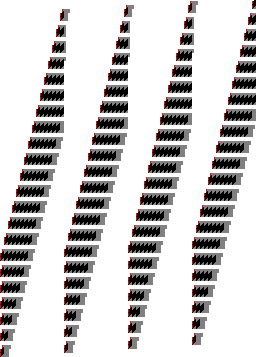
\includegraphics[width=0.4\textwidth]{st_diagrams/stencil7x7_column_4.png}};
        \draw [->] (image.south west) -- ++(2,0) node[right]{\footnotesize\textit{Time}};
        \draw [->] (image.south west) -- ++(0,2) node[rotate=90, above]{\footnotesize\textit{Address}};
    \end{tikzpicture}
    \caption{
        The spatial temporal diagram of a 7x7 stencil with a column of size 4 ordering.
        See section \ref{sec:st_analysis}.
    }
    \label{fig:st_stencil_column}
\end{figure}

The size of the cache needed $M_{size}$ can be approximated given the units per cache line $L$, column width $c$, stencil width $s_{w}$ and height $s_{h}$, and the number of active threads $t$. The required memory is independent of the size of the input data.

\[
    M_{size} = u \left(c + s_w\right) \left(s_h + \ceil{\frac{t}{c}}\right)
\]

Solving for $c$ gives an unneedly complex solution, so instead we approximate $M_{size}$ using the asymptote.

\[
    M_{size} = u \left(t + s_h \left(c + s_w\right)\right)
\]

Solving for column width $c$ gives 

\[
    c = \frac{M_{size} - u (s_h s_w + t)}{s_h u}
\]

The amount of fetches is similar to equation \ref{eq:stencil_tiling_fetches}, however, since we do not divide the work horizontally anymore, the number of cache line fetches is slightly lower:

\begin{equation}
    F \leq \ceil{\frac{I_w}{c}}\ceil{\frac{c + S_w}{L}} (I_h + S_h)
    \label{eq:stencil_column_fetches}
\end{equation}

\section{Matrix Multiplication}
Matrix multiplication can benefit from a column based approach due to many vertical reads.
Section \ref{sec:access_patterns} showed that continuous vertical reads are more expensive than continuous horizontal reads (streaming).
Therefore, we want to keep data that is read vertically in cache for as long as possible.
The naive implementation (section \ref{sec:matrix_naive}) showed that working on an entire row of outputs requires to load the whole $I_w \times D$ data
By limiting the horizontal space we work on, we can control what stays in case, increasing reuse.

\begin{figure}
    \centering
    \begin{tikzpicture}[scale=0.5]
        % Cached areas
        \draw[gray, pattern=north east lines, pattern color=gray!50] (2.5, 0.5) rectangle +(4, 8);
        \draw[gray, pattern=north east lines, pattern color=gray!50] (2.5,-3.5) rectangle +(4, 1);

        % Work areas
        \draw[gray, pattern=north west lines, pattern color=gray] ( 4.5, 0.5) rectangle +( 1, 8);
        \draw[gray, pattern=north west lines, pattern color=gray] ( 4.5,-3.5) rectangle +( 1, 1);
        \draw[gray, pattern=north west lines, pattern color=gray] (-0.5,-3.5) rectangle +(-8, 1);

        \draw[gray, dashed] (-0.5, -2.5) -- +(3, 0);
        \draw[gray, dashed] (-0.5, -3.5) -- +(3, 0);
        
        \draw[gray, dashed] (2.5, 0.5) -- +(0, -3);
        \draw[gray, dashed] (4.5, 0.5) -- +(0, -3);
        \draw[gray, dashed] (5.5, 0.5) -- +(0, -3);
        \draw[gray, dashed] (6.5, 0.5) -- +(0, -3);

        \draw ( 0.5,  0.5) rectangle +( 8,  8);
        \draw ( 0.5, -0.5) rectangle +( 8, -8);
        \draw (-0.5, -0.5) rectangle +(-8, -8);
    \end{tikzpicture}
    \label{fig:mm_cache_footprint}
    \caption{
        Calculating a single element in a matrix multiplication can exploit the cheaper memory accesses on the same cachelines. 
    }
\end{figure}

A matrix multiplication of $A \cdot B = C$ with $C$ being of size $I_w \times I_h$, and $A$ and $B$ being size $I_w \times D$ and $D \times I_h$ respectively, we compute the lower bound on the required cache by seperating the horizontal and vertical reads.

\begin{figure}[ht]
    \centering
    \begin{tikzpicture}[spy using outlines={rectangle, magnification=4,connect spies}]
        \node (image) at (0,0) {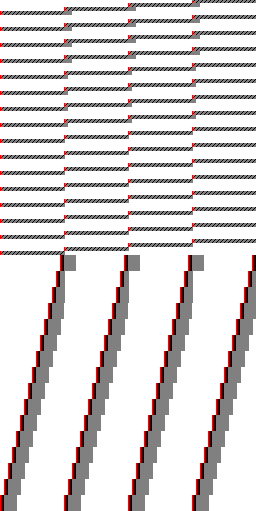
\includegraphics[width=0.25\textwidth]{st_diagrams/matrix_column_4.png}};
        \draw [->] (image.south west) -- ++(2,0) node[right]{\footnotesize\textit{Time}};
        \draw [->] (image.south west) -- ++(0,8.5) node[rotate=90, above left]{\footnotesize\textit{Memory Addresses}};

        \coordinate (p) at (0, 1);
        \coordinate (v) at (3.3, 2);
        \spy[width=2.4cm,height=4cm] on (p) in node [fill=white] at (v);
    \end{tikzpicture}
    \caption{
        The spatial temporal diagram of a matrix multiplication with a column of size 4 ordering.
        See section \ref{sec:st_analysis}.
    }
    \label{fig:st_matrix_column}
\end{figure}

The cachelines required $M_l$ for optimal cache usuage of a single row within a column of the matrix multiplication can be computed from the size of the matrices multiplied and the column width

\[
    M_{l} = \ceil{\frac{I_w}{L}} + I_h\ceil{\frac{c}{L}}
\]

Using cache size $M_{size}$ instead of cachelines gives a simpler equation, albeit less accurate

\[
    M_{size} = u I_h c 
\]

However the simpler approximation allows us to solve for the column width $c$ much more easier 

\[
    c = \frac{M_{size}}{u I_h}
\]
